\chapter{ProVerif analysis}


We analyze the protocols for authentication and signing using automatic protocol verification tool ProVerif. For each protocol, we first show the high-level representation of the protocol steps in a figure (copied from the initial architecture draft\footnote{\url{https://github.com/open-eid/browser-extensions2}}), and then list in detail the protocol steps as assumed in our ProVerif models.

Since a smart card uses different keys for authentication and signing, we model these two protocols separately, so that the analysis would be easier to ProVerif. For each protocol, we have several slightly different models, employing different protection profiles of Sec.~\ref{sec:protection_profiles}. The full ProVerif models can be found in the files
\begin{itemize}
\item\texttt{eid\_auth.pv} and \texttt{eid\_sign.pv} for the protocols without any protection mechanisms against MITM attacks;
\item\texttt{eid\_auth\_originValid.pv} and \texttt{eid\_sign\_originValid.pv} for the protocols with protection profile of Sec.~\ref{sec:origin_validation};
\item\texttt{eid\_auth\_certValid.pv} and \texttt{eid\_sign\_certValid.pv} for the protocols with protection profile of Sec.~\ref{sec:cert_validation};
\item\texttt{eid\_auth\_nonceSign.pv} and \texttt{eid\_sign\_nonceSign.pv} for the protocols with protection profile of Sec.~\ref{sec:challenge_signing}.
\end{itemize}
After downloading and installing ProVerif tool as explained in the ProVerif project page\footnote{\url{https://prosecco.gforge.inria.fr/personal/bblanche/proverif/}}, the analysis can be run as
\begin{verbatim}
   proverif -in pitype eid_auth.pv
   proverif -in pitype eid_auth_originValid.pv
   proverif -in pitype eid_auth_certValid.pv
   proverif -in pitype eid_auth_nonceSign.pv
   proverif -in pitype eid_sign.pv
   proverif -in pitype eid_sign_originValid.pv
   proverif -in pitype eid_sign_certValid.pv
   proverif -in pitype eid_sign_nonceSign.pv
\end{verbatim}

Note that the queries for which an attack is found are commented out from the models. Although ProVerif feedback is enough to understand the attack, it has some difficulties with reconstructing the trace, so it is better to execute these queries one by one.

\textbf{Disclaimer:} ProVerif can be used to verify security properties of high-level protocols, but it cannot discover errors in cryptographic primitives or implementation errors.


\section{Authentication Protocol}
\begin{figure}
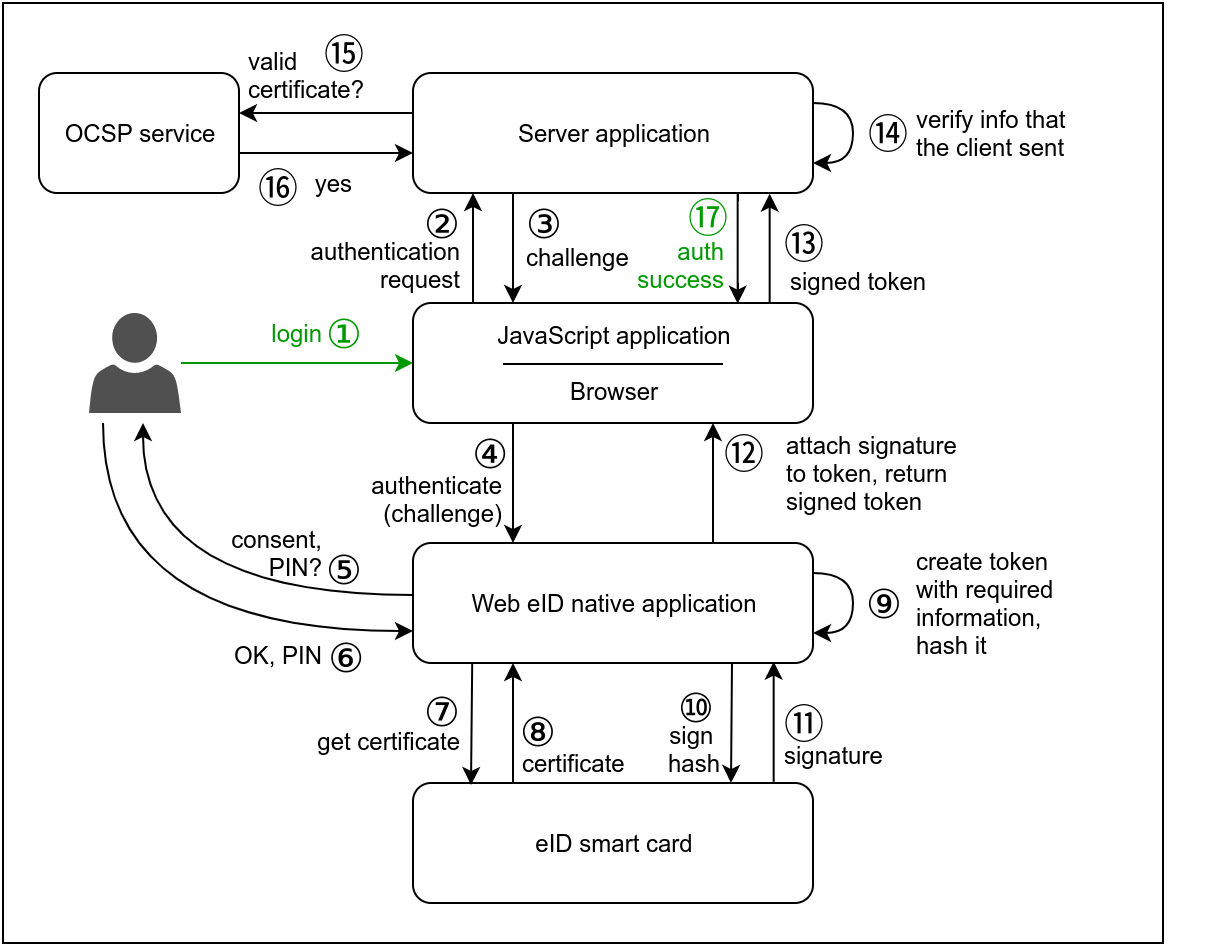
\includegraphics[width=\columnwidth]{img/authentication.png}
\caption{Web eID authentication diagram}\label{fig:auth}
\end{figure}

The eID authentication protocol is depicted in Figure~\ref{fig:auth}.

\subsection{Protocol model}\label{sec:authmodel}

\paragraph{Protocol parties:}

\begin{itemize}
\item User (U)   -- the user who wants to be authenticated;
\item Server (S) -- the server who authenticates;
\item Browser    -- the browser with JavaScript interpreter running in the user's local machine;
\item EID        -- Web eID native application running in the user's system;
\item SCard      -- smart card owned by the user;
\item Online Certificate Status Protocol (OCSP) service is not modeled as a separate party, and we assume that the Server has a black-box access to OCSP functionality.
\end{itemize}

\paragraph{Assumptions:}

We model a MITM attacker that intercepts communication in the public network. We ignore most of the possible internal threats such as learning the user's PIN or hacking into the OCSP service, which need to be treated separately. We only focus on threats coming from an external attacker. Denial-of-service attacks are also out of scope of ProVerif.

\begin{itemize}
\item The attacker intercepts network communication between the JS application and the Server. That is, we do not model interception on the level of the user's local machine.

\item The attacker may run an unbounded number of honest user and honest server sessions. He decides who communicates with whom in which order. He can himself control an unbounded number of malicious users and malicious servers.
    \begin{itemize}
    \item The attacker may control a user. To simplify modelling, the ProVerif code is written such that an attacker has issued a smart card for each malicious identity, and the corresponding certificate is recorded in the OCSP service. The attacker cannot obtain a card issued to an honest user.
    \item The attacker may control a server. TLS certificates are not strong, and the attacker can impersonate an honest server. We check whether obtaining a fake certificate is necessary for a particular attack.
     \end{itemize}

\item By default, the attacker has full control over the network (as it is usually modeled in ProVerif), and no one prevents him from getting all messages ever sent over transparent channels. To model the assumption that the attacker can only intercept the messages that are sent to his own IP addresses, we model DNS, which fixes an IP address for each identity, and creates a personal private channel for it. The attacker cannot read the messages destined to an honest party's IP unless it has been spoofed. We check whether DNS spoofing is necessary for a particular attack.

Alternatively, we could allow \emph{several} IP addresses for the same identity S. However, in our analysis, we assume that it is fine if the user connects to a different IP as far as the corresponding identity S is still correct. We also do not distinguish between the attacks related to adding a fake DNS record, or modifying an existing DNS record. Hence, we assume that one IP address per identity is sufficient.

%\item The EID service cannot be corrupted. Otherwise, the whole system would become insecure, as it would just learn the user's PIN and could do whatever if wants.

\item We assume that, once a TLS channel is established, it stays there until the end of authentication. We do not model the internal life of TLS and possible attacks on it. In practice, one should be careful with session resumption of TLS, as discussed in Sec~\ref{sec:mitm_risks_mitigations}.
\end{itemize}

\paragraph{Protocol steps:}We now describe the protocol steps in details. In the following, we use notation [$\cdot$] to denote optional values that are needed to be sent only for some settings.
\begin{enumerate}
\item\label{item:auth:step1} User inputs into browser the identity S of the server to connect with. Here the 'identity' is the same as the one stated in TLS certificate.
\begin{verbatim}
   U -> Browser: S
\end{verbatim}
\item\label{item:auth:step2} Browser makes a DNS lookup, finds the certificate of server S (which is potentially falsified), establishes TLS connection, and asks for a challenge
\begin{verbatim}
   Browser -TLS-> S: 'authRequest'
\end{verbatim}
\item\label{item:auth:step3} Server S generates a fresh nonce N and sends it to Browser. The message is marked as 'challenge', as N can be an arbitrary bitstring and has no special format. If we want to apply the protection method of Sec.~\ref{sec:challenge_signing}, we also require a signature NSign on N.
\begin{verbatim}
   S -TLS-> Browser: 'challenge', N, [NSign]
\end{verbatim}
\item\label{item:auth:step4} Browser sends to EID a request to meet the challenge. It also delivers the server hostname S, so that EID could display it to the user. If we choose to sign the server TLS certificate or the server's signature on challenge (i.e. apply protection profile of Sec.~\ref{sec:cert_validation} or Sec.~\ref{sec:challenge_signing}), we need to submit these as well.
\begin{verbatim}
   Browser -> EID: 'authRequest',S,N, [ServerCert, NSign]
\end{verbatim}
\item\label{item:auth:step5} EID prompts a PIN from User. In ProVerif model, we add S and N to the message, so that the inserted PIN can be linked to a particular authentication session. I.e. the response S,N,PIN cannot be used for another session S',N',PIN for S $\neq$ S' or N $\neq$ N'. In the next step, we discuss the necessity of actually displaying S and N to the user.
\begin{verbatim}
   EID -> User: S, N,'need_pin'
\end{verbatim}
\item\label{item:auth:step6} User inserts the PIN. EID application has to link the received PIN to the correct authentication session. In practice, if several sessions are running in parallel (e.g. another session is initiated by clicking on something by mistake), then the user should be aware of which session exactly he is approving. Ideally, we can display to the user the server identity S and the challenge N (or some other session ID derived from these two, e.g. a visual image) which he should verify against the values he sees in the 'correct' browser window. It may happen that a careless user does not perform this visual check, or there is some security environment that allows to re-use the PIN without user having to enter it again. In ProVerif model, we consider both possibilities, and we need to add S,N to the user's response if we want to link the inserted PIN to the correct session.
%User inserts the PIN. We assume that EID is able to link the received PIN with the correct S and N, and it is not possible to re-use the PIN. In our model, we consider also the case where the user does not perform a careful visual check before inserting the PIN, so adding S,N depends on this setting.
\begin{verbatim}
   User -> EID: PIN, [S,N]
\end{verbatim}
\item\label{item:auth:step7} EID gets the certificate out of the smart card.
\begin{verbatim}
   EID -> SCard: 'getCertificate()'
\end{verbatim}
\item\label{item:auth:step8} SCard returns the certificate UserCert to anyone who asks for it, without a PIN.
\begin{verbatim}
   SCard -> EID: UserCert
\end{verbatim}
\item\label{item:auth:step9} EID computes a token T = hash(T'), where T' depends on the protection profile. Let ServerCert be Server's TLS certificate (possibly fake) that has been chosen on User's side to establish TLS connection. The value of T' can be one of the following.

\begin{itemize}
\item hash(N) if no MITM protection methods are used.
\item hash(S,N) for the protection method of Sec.~\ref{sec:origin_validation}.
\item hash(S,N,ServerCert) for the protection method of Sec.~\ref{sec:cert_validation}. In a real application, the server certificate SHA-256 fingerprint is used instead of the full certificate. This does not make any difference to ProVerif model, as we do not model details of cryptographic primitives and treat all hashes as ideal.
\item hash(S,N,NSign) for the protection method of Sec.~\ref{sec:challenge_signing}. If we do not add NSign to the token, then the Server will not be able to check later whether the signature received by the User was correct, and MITM can sign N himself with his own TLS key.
\end{itemize}


\item\label{item:auth:step10} EID forwards the PIN to SCard and asks for a signature on T. A unique identifier SID links the output of SCard to a particular input to avoid messing up signatures of different messages. SID is a part of ProVerif model that is not explicitly generated in the real protocol. In practice, EID application should match the signature it receives from SCard to the appropriate authentication session,  even if several sessions are running in parallel.
\begin{verbatim}
   EID -> SCard: SID, T, PIN
\end{verbatim}
\item\label{item:auth:step11} The SCard computes the signature Sign = sign(SK,T) on T, where SK is the user's secret key stored in SCard, and sends it to EID.
\begin{verbatim}
   SCard -> EID: SID, Sign
\end{verbatim}
\item\label{item:auth:step12} EID attaches Sign to the token T and forwards these to Browser. EID also sends the user certificate UserCert, which can be later be verified against OCSP service.
\begin{verbatim}
   EID -> Browser: UserCert, T, Sign
\end{verbatim}
\item\label{item:auth:step13} Browser forwards received data to the Server through TLS pipe.
\begin{verbatim}
   Browser -TLS-> S: UserCert, T, Sign
\end{verbatim}
\item\label{item:auth:step14} The Server verifies the signature and the values stored in T.

\item\label{item:auth:step15} The Server consults the OCSP service whether the certificate is valid.

\item\label{item:auth:step16} The Server proceeds only of OCSP has approved the certificate.

\item\label{item:auth:step17} The Server notifies Browser that the authentication succeeded. The 'ok' message should be accompanied with the user name A and the nonce N for which the agreement has been established. These values prevent the attacker from replaying 'ok' message from some previous session. The user name A can be removed if TLS itself ensures that the message of S that is meant for Bob will not be accepted by Alice. In ProVerif models, we do not assume the latter by default, as the protocol works with transparent TLS, where no shared key has been established yet.
\begin{verbatim}
   Server -TLS-> Browser: A, N, 'ok'
\end{verbatim}
\item\label{item:auth:step18} The browser displays to the user a message 'ok'. This additional message is needed for modeling purpose, to verify the consistency of views of the User and the Server.
\begin{verbatim}
   Browser -> User: S, 'ok'
\end{verbatim}
\end{enumerate}

\subsection{Security analysis}

In the model, we consider relations between the following events.

\begin{itemize}
\item \texttt{event honest(A)} -- the secret key of party A is not known to the attacker.
\item \texttt{event honestPK(S,PK)} -- PK is the actual public key of the server S.

\item \texttt{event fakeServerCert(S)} -- attacker has obtained a fake TLS certificate of S.
\item \texttt{event dnsPoisonedName(S)} -- attacker modified the DNS table entry of the party S.
\item \texttt{event carelessUser(A)} -- the user ignores messages accompanying PIN request.

\item \texttt{event signedBySCard(A,M)} -- the smart card of party A has signed a message M.

\item \texttt{event beginUser(A,S)} -- the user A started establishing a session with S.
\item \texttt{event endUser(A,S)}   -- the user A has finished authentication to S.

\item \texttt{event endServer(A,S,N)} -- the server S has accepted authentication of A w.r.t. challenge N.
\item \texttt{event endJS(A,S,N,PK)} -- the JS interpreter at A's side has finished session with S w.r.t. challenge N, where PK is the public key of S used to establish TLS connection.

\item \texttt{event tlsJS(A,S,TlsNonce)} -- the JS interpreter at A's side established a TLS session defined by TlsNonce with S.
\item \texttt{event tlsServer(A,S,TlsNonce)}-- the server S established a TLS session defined by TlsNonce with JS interpreter at A's side.
\end{itemize}


We will further mark with '+' successful security proofs (ProVerif answers TRUE), and with '-' the disproofs (ProVerif answers FALSE, i.e. an attack trace is found). We group the ProVerif queries according to security goals. For each query, we first display the straightforward ProVerif statement, based on the events listed above, and then explain what it means.

In the following, we use the variable $T$ to denote the token signed by the user. The exact structure of this token depends on the protection profile. If the answer to the query turns out to depend on the choice of $T$, we mark it as $\pm$ and discuss it.

We are going to analyze whether an honest user A or an honest server S can be impersonated. We assume that an honest party always behaves according to the protocol rules, and we do not aim to protect a party that does not follow the protocol. A misbehaving party is treated as corrupted, and ProVerif does take into account the harm that it may cause to some other party. The attacker is allowed to control any number of servers and any number of users, so the model is not constrained to interactions between an honest user A and an honest server S.

\paragraph{Can attacker impersonate A to S?}

\begin{itemize}
\item[+] \texttt{query A : party, S : party, N : bitstring,\\
                 NSign : signature, PKS : pkey;\\
                 event(honest(A)) \&\& inj-event(endServer(A,S,N))\\
                 ==> inj-event(signedBySCard(A,$T$)).}

If the server S thinks that he established a connection with an honest user A with session nonce N, then indeed the smart card of A was used to sign the token $T$ of that session. This proves that authentication will not work without smart card signing the challenge. This does not yet prove that the user A is aware of what has been signed with their card.

\item[--] \texttt{query A : party, S : party, N : bitstring;\\
                  event(honest(A)) \&\& event(endServer(A,S,N))\\
                  ==> event(beginUser(A,S)).}

If the server S thinks that he established a connection with an honest user A with session nonce N, but the PIN is not linked to the server hostname, then it may be a replay attack where A actually does not intend to authenticate to S.

\item[$\pm$] \texttt{query A : party, S : party, N : bitstring;\\
                 event(honest(A)) \&\& inj-event(endServer(A,S,N))\\
                 ==> inj-event(beginUser(A,S)) || event(carelessUser(A)).}

If the server S thinks that he established a connection with an honest user A with session nonce N, then unless the user's PIN has been inserted into a wrong window, the user A has indeed wanted to connect to S. This fact depends on the used protection mechanism.
\begin{itemize}
\item[--] If no protection mechanisms are applied, then the response of A is not linked to any server identity, and the challenge N could have been forwarded by a MITM attacker.
\item[+] If we apply the protection method of Sec.~\ref{sec:origin_validation}, then the signature of A on the origin prevents server from accepting messages that A planned for some other origin.
\item[+] The method of Sec.~\ref{sec:cert_validation}   contains the origin as well, and works similarly to Sec.~\ref{sec:origin_validation}.
\item[+] The method of Sec.~\ref{sec:challenge_signing} contains the origin as well, and works similarly to Sec.~\ref{sec:origin_validation}.
\end{itemize}
If ProVerif answers TRUE to this query, the liveness of A is proven. However, this does not yet prove that A is indeed on the other end of the TLS pipe.

\item[$\pm$] \texttt{query A : party, S : party, TlsNonce : bitstring;\\
                 event(honest(A)) \&\& event(tlsServer(A,S,TlsNonce))\\
                 ==> event(tlsJS(A,S,TlsNonce)).}

If the server authenticates A, then A is indeed on the other end of TLS pipe. This fact depends on the used protection mechanism.
\begin{itemize}
\item[--] If no protection mechanisms are applied, then the response of A is not linked neither to any server identity nor any TLS pipe.
\item[$\pm$] If we apply the protection method of Sec.~\ref{sec:origin_validation}, then a MITM attacker that gets a fake certificate of S may forward the signed challenge of A to S through a separate TLS connection. For this, the attacker needs to intercept the message that A intended for S. If the attacker can intercept only those messages that are destined to an IP address controlled by it, then everything is fine as far as DNS table has not been poisoned (ProVerif will answer TRUE if we add \texttt{|| event(dnsPoisonedName(S))} or \texttt{|| event(fakeServerCert(S))} to the right-hand-side). In practice, we would still not be protected e.g. against malware that intercepts all outgoing messages, or an attacker located at the LAN gateway.
\item[+] If we apply the protection method of Sec.~\ref{sec:cert_validation}, then the signature of A on the certificate used in TLS prevents server from accepting a TLS connection that originates from an attacker. We assume that the Server and the Attacker do cannot share the same certificate, and there would still be an attack if the attacker managed to steal the private key corresponding to the TLS certificate owned by the Server.
\item[+] The protection method of Sec.~\ref{sec:challenge_signing} works similarly to the method of Sec.~\ref{sec:origin_validation}. Instead of signing the TLS certificate directly, A signs the signature on challenge that it received from S, which is indirectly linked to TLS certificate as well.
\end{itemize}

\end{itemize}

We conclude that, as far as the additional protection methods of Sec.~\ref{sec:protection_profiles} are applied, the server can be convinced that the user is alive, and indeed sits on the other end of the TLS pipe.

\paragraph{Can attacker impersonate S to A?}

\begin{itemize}

\item[--] \texttt{query A : party, S : party, PK : pkey, N : bitstring;\\
                  event(honest(S)) \&\& event(endJS(A,S,N,PK))\\
                  ==> event(endServer(A,S,N)).}

Without A checking the public key PK or the IP address of the server S against a trusted source, the attacker may easily impersonate S by presenting a fake TLS certificate.

\item[+] \texttt{query A : party, S : party, PK : pkey, N : bitstring;\\
                 event(honestPK(S,PK)) \&\& inj-event(endJS(A,S,N,PK))\\
                 ==> inj-event(endServer(A,S,N)).}

If the browser is convinced that the server's public key used in generation of TLS was indeed the honest server's one (e.g. confirmed using side-channels), then the nonce N was indeed generated by the server S that owns the corresponding secret key PK. So even though the user might not know which session exactly was accepted, the browser does know it.

\item[+] \texttt{query A : party, S : party, PK : pkey, N : bitstring;\\
                 event(honest(S)) \&\& inj-event(endJS(A,S,N,PK))\\
                 ==> inj-event(endServer(A,S,N)) || event(dnsPoisonedName(S)).}

If CA is not trusted, then the browser may instead read server's IP address from a trusted DNS table. This works as far as there is no DNS poisoning or message redirection.

\item[+] \texttt{query A : party, S : party, PK : pkey, N : bitstring;\\
                 event(honest(S)) \&\& event(endUser(A,S))\\
                 ==> event(endServer(A,S,N))|| event(fakeServerCert(S)).}

As far as the server has not been impersonated by fake certificates, the user that has received an authentication approval response can be sure that the real server approved at least one of the sessions that the user attempted to establish.

\item[--] \texttt{query A : party, S : party, PK : pkey, N : bitstring;\\
                 event(honest(S)) \&\& inj-event(endUser(A,S))\\
                 ==> inj-event(endServer(A,S,N)) || event(fakeServerCert(S)).}

Let us now see whether the \emph{injective} variant of the previous agreement query holds, i.e. is each server's acceptance is followed by \emph{at most one} user's acceptance. If there are several sessions running in parallel, the user may get a wrong opinion which one of them exactly was run with the true server S. This is because we do not show the nonce  to the user. This is not a problem, since it does not matter for the user which one of the sessions was accepted. From the previous queries, we see that the browser does know what the correct session ID is.

\end{itemize}

We conclude that the attacker cannot impersonate S unless he obtains at once a fake certificate and corrupts the DNS service. %Alternatively, if the server obtains an additional \emph{strong} certificate that cannot be faked, then it can use the corresponding key to sign the messages of steps (\ref{item:step3}) and (\ref{item:step17}), thus applying a variant of protection method described in Sec.~\ref{sec:challenge_signing}. Note that if the server signs \emph{only} the challenge at step (\ref{item:step3}), then a MITM attacker will stop forwarding messages to S and continues playing S to A, so signing (\ref{item:step17}) is important as well. It is also important that the additional signature is generated using a more trustworthy (or at least different) certificate, so that the attacker cannot just generate the additional signature of S himself.

\paragraph{Can the attacker misuse the smart card, which may potentially endanger other applications that use the same card?}

\begin{itemize}
\item[+] \texttt{query A : party, S : party, N : bitstring,\\
                 NSign : signature, PKS : pkey;\\
                 event(signedBySCard(A,$T$))\\
                 ==> event(beginUser(A,S,N)) || event(carelessUser(A)).}

If a smart card has signed something in scope of our protocol, then the user is aware of it, unless the PIN has been inserted into a wrong window. Note that the events are not injective, so if the user has approved signing a message M once, it does not yet mean that the same message can be signed multiple times without user being aware.

\item[--] \texttt{query A : party, S : party, N : bitstring,\\
                  NSign : signature, PKS : pkey;
                  event(honest(A))\&\& event(honest(S))\&\& inj-event(signedBySCard(A,$T$))\\
                  ==> inj-event(beginUser(A,S,N)) || event(carelessUser(A)).}

Let us now see whether the \emph{injective} variant of the previous agreement query holds, i.e. is each PIN insertion followed by \emph{at most one} signing. We see that, even if we link the user's PIN to a particular server hostname S and nonce N, it can be used multiple times to sign exactly the same message. This could potentially make some signature forging attacks easier by outputting signatures of the same message with different randomness. This issue seems more like ProVerif incompleteness than a real attack, as in reality an honest EID would prompt the PIN again each time, even if the message to be signed is exactly the same. ProVerif assumes that, once a message was sent to some channel, it can be used an unbounded number of times.
\end{itemize}

We conclude that generation of fake signatures is not possible without user being aware of that, as far as the PIN has been linked to the correct session.

\section{Signing Protocol}
\begin{figure}
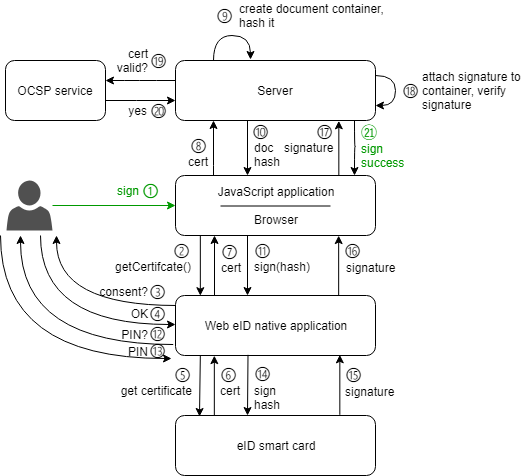
\includegraphics[width=\textwidth]{img/signing.png}
\caption{Web eID signing diagram}\label{fig:sign}
\end{figure}

The eID signing protocol is depicted in Figure~\ref{fig:sign}.

\subsection{Protocol model}

As the protocol structure is very similar to that authentication protocol, the set of parties and the assumptions are the same as in Sec.~\ref{sec:authmodel}.

\paragraph{Protocol steps:}

\begin{enumerate}
\item User inputs into Browser the identity S of the server to connect with. Here the 'identity' is the same as the one stated in TLS certificate. 
\begin{verbatim}
   U -> Browser: S
\end{verbatim}
\item Browser queries from EID the certificate by sending a constant message.
\begin{verbatim}
   Browser -> EID: 'getCertificate()'
\end{verbatim}
\item EID shows the constant message 'consent' to the user to verify their presence.
\begin{verbatim}
   EID -> U: 'consent'
\end{verbatim}
\item User confirms the consent. We note that the messages are not linked to particular S with which User tries to connect. Since the same certificate is used in all sessions, and it is public, this is not a problem.
\begin{verbatim}
   U -> EID: 'ok'
\end{verbatim}
\item EID gets the certificate out of the smart card.
\begin{verbatim}
   EID -> SCard: 'getCertificate()'
\end{verbatim}
\item SCard returns the certificate UserCert to anyone who asks for it, without a PIN.
\begin{verbatim}
   SCard -> EID: UserCert
\end{verbatim}
\item EID forwards UserCert to Browser.
\begin{verbatim}
   EID -> Browser: UserCert
\end{verbatim}
\item Browser makes a DNS lookup, finds the certificate of server S (which is potentially fake), establishes TLS connection, and sends UserCert to S.
\begin{verbatim}
   Browser -TLS-> Server: UserCert
\end{verbatim}
\item Server creates a document container and hashes it with a fresh randomness, creating a nonce N. At this point, server has not yet verified UserCert.

\item Server sends fresh randomness N to Browser. In reality, N would be a randomized document container, but we model it just as a random number. Including the randomness into document container is important to avoid replay attacks. If we want to apply the protection method of Sec.~\ref{sec:challenge_signing}, we also require a signature NSign on N.
\begin{verbatim}
   Server -TLS-> Browser: 'challenge',N, [NSign]
\end{verbatim}
\item Browser asks EID for a signature. We need to deliver the server identity S as well, as it will be displayed to the user. If we choose to sign one the server TLS certificate, or the server's signature on challenge, we need to submit these as well.
\begin{verbatim}
   Browser -> EID: 'authRequest',S,N, [ServerCert, NSign]
\end{verbatim}
\item EID prompts a PIN from the User. In ProVerif model, we add S and N to the message, so that the inserted PIN can be linked to a particular authentication session. I.e. the response S,N,PIN cannot be used for another session S',N',PIN for S $\neq$ S' or N $\neq$ N'.
%EID prompts a PIN from the User. It is important to display to the user the server name S, to avoid signing challenge of some other server. Displaying N does not help much, as it looks as a completely random value to the user anyway. Including N is important if the contents of the document container are important, and e.g. the user may decide to refuse to sign even an honest server's challenge. In ProVerif model, adding N to the message is needed for linking the PIN response to a particular authentication session. I.e. the response S,N,PIN cannot be used to generate a signature for another session S,N',PIN for N $\neq$ N'.
\begin{verbatim}
   EID -> User: S,N,'need_pin'
\end{verbatim}
\item User sends PIN to the EID application, which has to link it to the correct authentication session. Similarly to authentication protocol, we need to add S,N to the user's response if we want to link the inserted PIN to the correct session. Including N is more important for the signing protocol, since N depends on the contents of the document container, and the user should see what he is signing even if the server identity S is correct.
\begin{verbatim}
   User -> EID: PIN, [S,N]
\end{verbatim}
\item Similarly to the authentication protocol, EID constructs a token T according to particular protection profile, and a unique identifier SID links the output of SCard to a particular input to avoid messing up signatures of different messages.
\begin{verbatim}
   EID -> SCard: SID, T, PIN
\end{verbatim}
\item The SCard computes the signature Sign = sign(SK,T) on T, where SK is the user's secret key stored in SCard, and sends it to EID.
\begin{verbatim}
   SCard -> EID: SID, Sign
\end{verbatim}
\item EID forwards the signature Sign to Browser.
\begin{verbatim}
   EID -> Browser: Sign
\end{verbatim}
\item Browser forwards the signature Sign to the Server. We label this message as 'userSignature', since a signature itself is a bitstring which does not have a specific format, and can be confused with other messages.
\begin{verbatim}
   Browser -TLS-> S: 'userSignature', Sign
\end{verbatim}
\item The Server verifies the signature and attaches it to the container.

\item The Server consults the OCSP service whether the certificate is valid.

\item The Server proceeds only of OCSP has approved the certificate.

\item The Server notifies the Browser that the signing succeeded.
\begin{verbatim}
   Server -TLS-> Browser: A, N, 'ok'
\end{verbatim}
\item The browser displays to the user a message 'ok'. This additional message is needed mainly for modeling purpose, to verify the consistency of views of an honest User and an honest Server.
\begin{verbatim}
   Browser -> User: S, 'ok'
\end{verbatim}
\end{enumerate}

\subsection{Security analysis}

As the protocol structure is very similar to that of authentication protocol, we run the same ProVerif queries. The answers to these queries are similar to the authentication protocol, sharing same strengths and weaknesses. There are however some small differences.

\begin{itemize}

\item Signing the origin and/or the TLS certificate (protection profiles of Sec.~\ref{sec:origin_validation} and Sec.~\ref{sec:cert_validation}) help to prove that, if the server authenticates A, then A is indeed on the other end of TLS pipe. The advantage of signing protocol is that it finishes after the last step, so we do not need to worry what happens next, and whether A has indeed been on the other end of the TLS pipe. The goal of the protocol is still achieved as far as the real A signed the document that the server wanted it to sign, even if the MITM attacker forwarded all messages.

\item If the document container to be signed contains private information, then it may indeed be important who is on the other side of TLS. In this case, A would need to be authenticated \emph{before} the document container hash is sent out, which would be something different from the protocol of Fig.~\ref{fig:sign}.
\item
Differently from authentication, it can now be important to see which challenge N exactly was signed. That is, when the user inserts PIN, he sees the contents of the signed document container through the browser, and not through eID interface. While it is impractical to show the entire signed document through eID window, the value N is anyway not the document itself, but a hash, which could possibly be displayed by eID as well to reduce trust in browser. Again, since the user cannot compute the hash from visually observed document, they would need to trust the browser to do this automatically, or download the document and compute the hash by some independent tool, which would already make the ceremony very different from what we had initially. Visual verification of a hash can also be challenging, as small difference in some symbols can easily remain unnoticed.
\end{itemize}

\newcommand{\implies}{\Rightarrow}
\newcommand{\dns}{\mathsf{A_{IP}}}
\newcommand{\tls}{\mathsf{A_{CERT}}}
\section{Summary}

Table~\ref{table:proverifsummary} summarizes the capabilities of an external attacker for different protection profiles for both the authentication and the signing protocols. To make the representation more compact, we denote the event ``\emph{the attacker is able to intercept messages destined to the server}'' as $\dns$, and ``\emph{the attacker can obtain a fake TLS certificate}'' as $\tls$.

We note that we do not consider the problems related to the assumption that the user thoroughly reads the hash that he is going to sign, and compares it carefully against the hash of the actual document that he wanted to get signed. Problems on user side are out of scope of an external attacker analysis.

\begin{table}[ht]
\center
\begin{tabular}{| l | l | l |}
\hline
protection profile &  user impersonation & server impersonation                \\
\hline
none              & NOT OK               & $\neg\dns\vee\neg\tls\implies$OK \\
origin signing  (Sec.~\ref{sec:origin_validation})    & $\neg\dns\vee\neg\tls\implies$OK & $\neg\dns\vee\neg\tls\implies$OK \\
cert signing (Sec.~\ref{sec:cert_validation})       & OK                   & $\neg\dns\vee\neg\tls\implies$OK \\
challenge signing (Sec.~\ref{sec:challenge_signing}) & OK               & $\neg\dns\vee\neg\tls\implies$OK \\
\hline
\end{tabular}
\caption{Summary of ProVerif analysis for different protection profiles, where $\dns$ denotes that the attacker can poison DNS tables, and $\tls$ that the attacker can obtain a fake certificate for an honest server's name.}\label{table:proverifsummary}
\end{table}
